\section{Method Validation}\label{sec:validation}

Throughout, \emph{preregistered} denotes an analysis plan prospectively frozen in the version-controlled project repository before the corresponding execution, with the frozen commit identifier recorded in run metadata.

Before applying FALI to pretrained models, we tested whether the intervention game recovers known factors in controlled systems and reproduces ordinary transformer computation at its two natural endpoints. These preregistered checks validate implementation semantics rather than learned-model mechanisms. Figure~\ref{fig:validation} summarizes the tests.

\begin{figure*}[t]
\centering
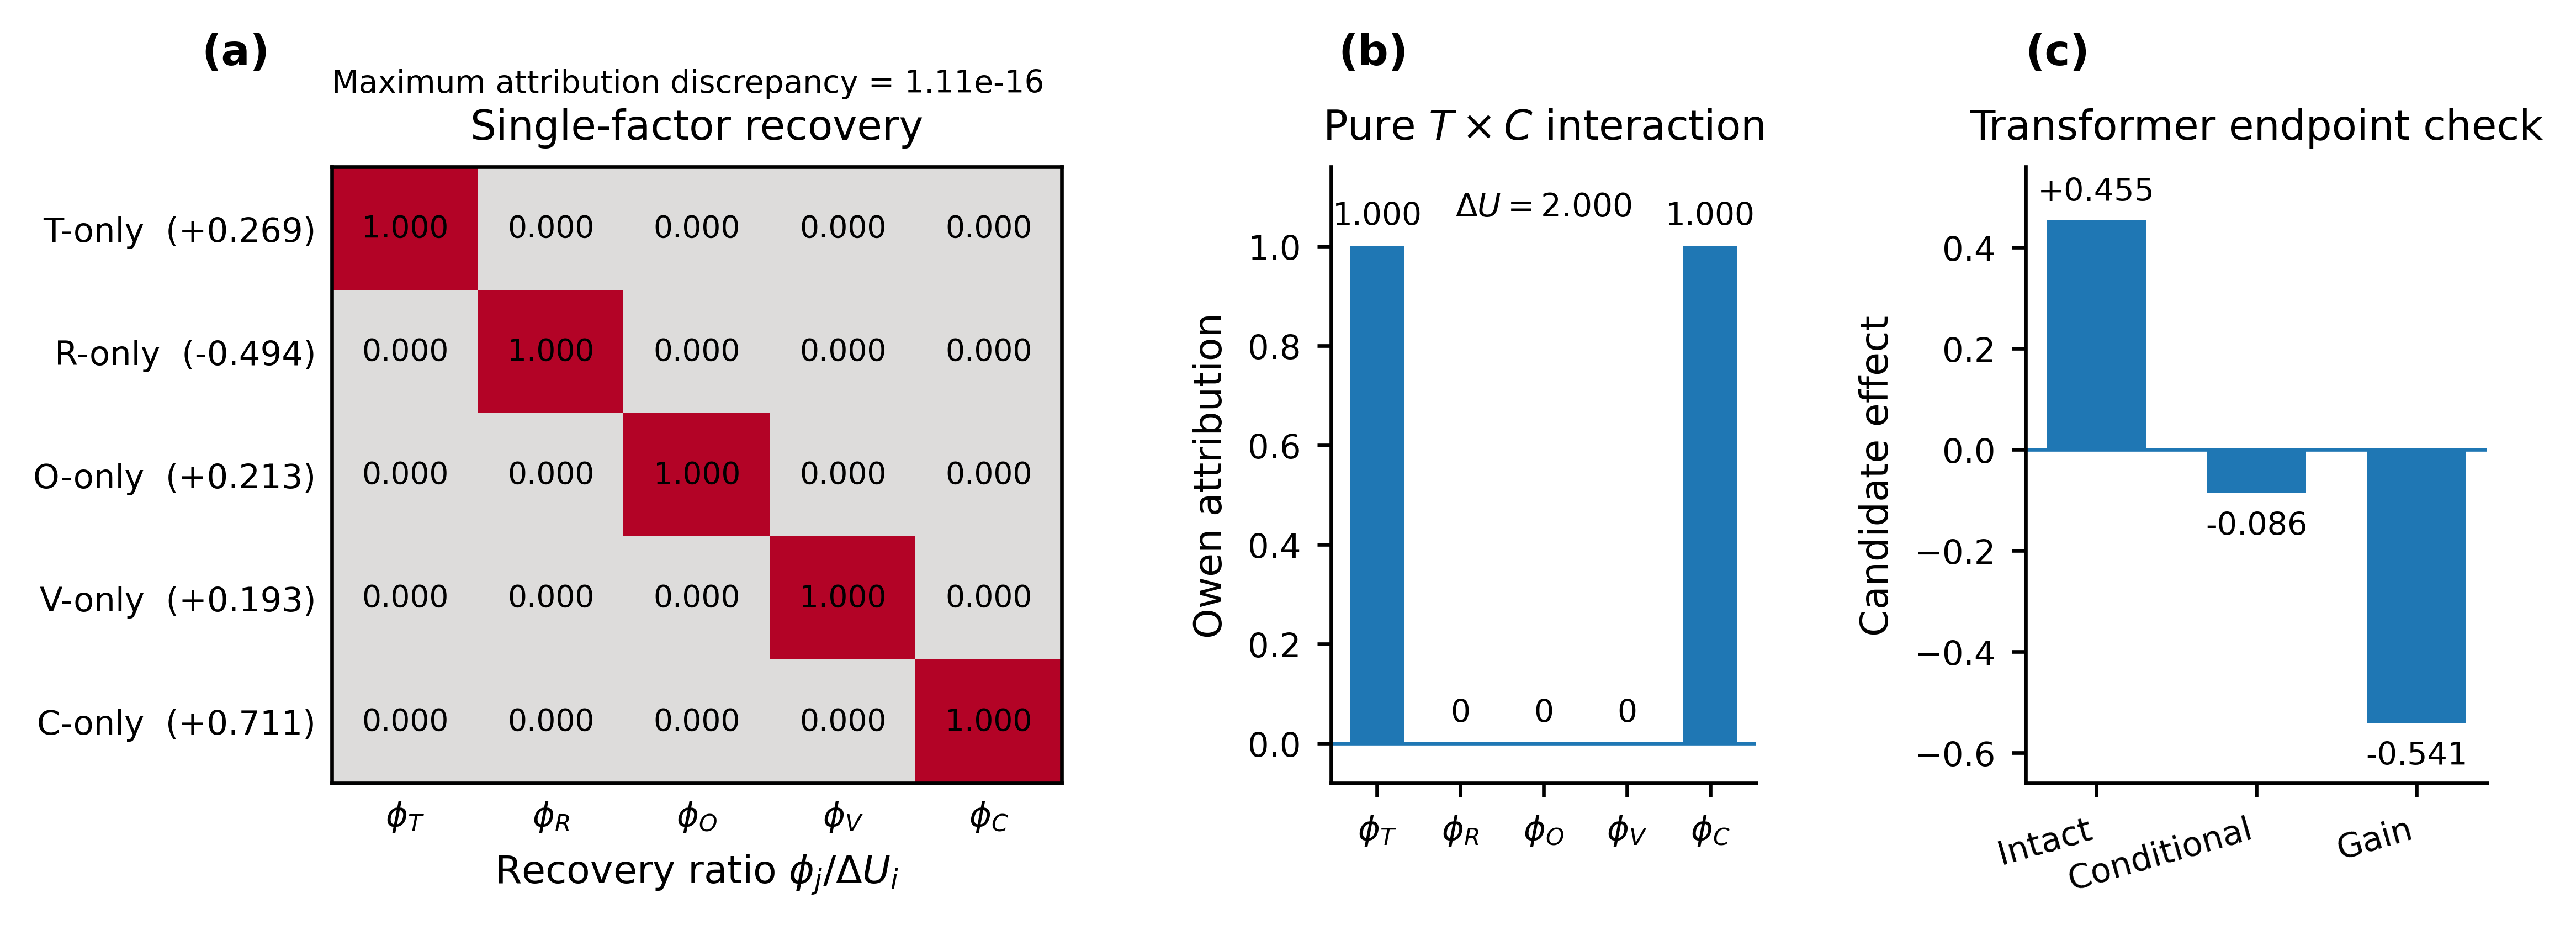
\includegraphics[width=\textwidth]{figures/Fig3.png}
\caption{\textbf{Controlled validation recovers known factors, interaction allocation, and transformer endpoint identities.}
(a) In five deterministic single-factor systems, the manipulated factor receives the full endpoint change: each row shows the recovery ratio $\phi_j/\Delta U_i$, with the raw injected $\Delta U_i$ given beside the row. The maximum attribution discrepancy is $1.11\times10^{-16}$.
(b) A pure $T\times C$ construction with $\Delta U\approx2$ yields the analytically expected Owen split $\phi_T\approx1$ and $\phi_C\approx1$, with $R,O,V=0$.
(c) In the randomly initialized two-layer TransformerLens validation model, independently measured intact effect, conditional effect, and conditional gain are $0.455046$, $-0.085684$, and $-0.540729$, respectively, and the corresponding FALI endpoint cells reproduce them exactly at recorded precision. Reconstruction, leakage, and model-level quotient residuals are zero at recorded precision.
These are implementation and controlled-ground-truth checks, not evidence that mixed FALI hybrids are unique natural model pathways.}
\label{fig:validation}
\end{figure*}


\subsection{Analytical and synthetic ground truth}\label{sec:synthetic}

We constructed deterministic attention systems containing causal scores, masked softmax, values, $z=PV$, and a context-specific readout, and evaluated all 32 FALI cells. In five single-channel cases, only the manipulated factor received attribution: for example, the target-only system gave $\Delta_h=0.268952$ with $\phi_T=0.268952$, and the rival-only system gave $\Delta_h=-0.494100$ with only $\phi_R$ nonzero. The $O$, $V$, and $C$ cases behaved analogously; the largest attribution error was $1.11\times10^{-16}$. Panel (a) of Fig.~\ref{fig:validation} shows this factor-isolation recovery directly.

A separate pure $T\times C$ construction had $\Delta_h\approx2$ with no isolated marginal effect and yielded the analytically expected Owen split $\phi_T\approx1$, $\phi_C\approx1$, with $R,O,V=0$. All-$A$ and all-$B$ hybrids reconstructed their endpoints exactly at recorded precision, and collapsing $T,R,O$ into SCORE reproduced the corresponding three-player SCORE/VALUE/CONTEXT decomposition with maximum discrepancy $1.11\times10^{-16}$. Panel (b) of Fig.~\ref{fig:validation} shows the expected interaction allocation.

\subsection{Transformer implementation invariants}\label{sec:implementation-validation}

We then repeated the mechanical checks in a randomly initialized two-layer TransformerLens model (two heads per layer, $d_{\mathrm{model}}=32$, $d_{\mathrm{head}}=16$, $d_{\mathrm{mlp}}=64$, context length 8, vocabulary 48), evaluated in FP32 on CPU with seed 4242. Masked softmax reconstructed cached intact and perturbed attention patterns exactly at recorded precision, pattern--value multiplication reconstructed candidate $z$, masked coordinates received zero probability, and batch-specific $T/R/O$ partitions had one target coordinate, zero overlap, and complete valid-score coverage per example.

Independent ordinary forward passes gave intact effect $0.455046$, conditional effect $-0.085684$, and conditional gain $-0.540729$; the corresponding FALI endpoint cells reproduced all three with zero recorded discrepancy. Full candidate-$z$ injection left non-candidate heads unchanged, and large perturbations to the candidate's live query computation, value computation, or both produced zero recorded leakage once $z$ was overwritten. The model-level fine game and collapsed SCORE/VALUE/CONTEXT quotient also agreed exactly. Panel (c) of Fig.~\ref{fig:validation} reports the independent endpoint values; reconstruction, leakage, and model-level quotient discrepancies are zero at recorded precision.

These checks establish factor isolation, structural masking, endpoint recovery, intervention isolation, and coarse--fine reconciliation for the implemented pipeline. They do not establish that the factorization is unique, that mixed hybrids are on-manifold, or that a large attribution identifies a unique natural causal pathway; those interpretation limits remain explicit in Section~\ref{sec:limitations}.
